\documentclass{article}

\usepackage{graphicx}
\usepackage{tikz}
\usetikzlibrary{shapes.geometric, arrows} 
\usepackage{hyperref}
\hypersetup{
    colorlinks=true,
    linkcolor=blue,
    filecolor=magenta,      
    urlcolor=cyan,
    pdftitle={Overleaf Example},
    pdfpagemode=FullScreen,
}
\usepackage{titlesec}
\usepackage{geometry}
 \geometry{
 a4paper,
 total={170mm,257mm},
 left=20mm,
 top=20mm,
 }

%flowchart
\tikzstyle{startstop} = [rectangle, rounded corners, minimum width=3cm, minimum height=1cm, text centered, draw=black, fill=red!30]
\tikzstyle{io} = [trapezium, trapezium left angle=70, trapezium right angle=110, minimum width=3cm, minimum height=1cm, text centered, draw=black, fill=blue!30]
\tikzstyle{process} = [rectangle, minimum width=3cm, minimum height=1cm, text centered, draw=black, fill=orange!30]
\tikzstyle{decision} = [diamond, minimum width=3cm, minimum height=1cm, text centered, draw=black, fill=green!30]
\tikzstyle{arrow} = [thick,->,>=stealth]

\title{Unit 15 LO2}
\author{Chris}
\date{}

\begin{document}

\maketitle
\tableofcontents
\break

\section{P3 Create a design for an identified game concept}
We have been tasked in the previous Units to create a game for a food retailer. They are a fresh and modern company who are aware of moderen digital marketing techniques.
They are clear that they want to have a game developed which will be used as a part of their advertising campaigns. To that end they want to have a game developed that incorporates their branding and mascot, a food ninja.
The artifacts in the game must relate to their fast food outlets and the gameplay must be fun and engaging and reflect their healthy attitudes to food. 

The game is to be targetted at a younger audience and should have a an easy to pickup layout, meaning that the game play should be something most players will have played previously. To that end a platformer has been requested. 

\subsection{Game elements}
\subsubsection{Navigation}
The navigation in the game is done by providing important information to the player to the player by either using a Heads Up Display(HUD) for example compasses,maps or arrow signs. Both of these methods are helpful in games and their use depends on game's genre and how the game designers want the player to experience the game.

The HUD said by Greg Wilson in the article \textit{Off With Their HUDs} described HUD as "A collection of persistent onscreen elements whose purpose is to indicate player status. HUD elements can be use to show, among many other things, how much health the player has, in which direction the player is heading, or where the player ranks in a race" 



\subsubsection{Scoring}
Scoring in games are key component of game mechanics and it provides a mechanic where the players get rewarded with point value whenever they accomplish a task in the game.   
In this game the scoring will be based upon the collection of sweets that our client, the food producer creates. Thier mascot, a ninja will run swideways on the platformer and will need to avoid or defeat various monsters to be able to continue. As the ninja continues to move they will encounter various sweets that will increase their score, some of these sweets will also be dropped by the monsters which have been killed.

\subsubsection{Movement}
Moving a character is so common in games that players and designers often take it for granted. However, while it can be tempting to use the default movement options in a game engine, designing great movement can make simply controlling a character fun. 
Movement of the character in this game should be verty straightfoward, as this is a traditional 2D platformer the main character will need to
/begin{itemize}
/item Move left
/item Move right
/item Jump
/item Duck / Hide
/end{itemize}

It would be easy to add other actions such as adding combos that build up actions like Mortal Kombat or Super Smash Brothers but as the remit for this game is something which is familar we will stick with the basic movements for the first demo to the customer.

The controls will also default to the standard WASD controls but we will add a configuration page so that users can remap the controls if they want to.

\subsubsection{Interaction/Controls}
three main principles for good game controls are:
\begin{itemize}
	\item Accessibility - the controls should be easy to learn and use, and take into account physical and cognitive limitations
	\item Intent Communication - the controls should communicate the player's intent in a way the player expects and create a feeling of full control
	\item Expression Space - the controls should give the player enough expression so that they players can master while also keep a sufficient level of variety.
\end{itemize}

Accessibility 
If we want our controls to be easy to learn and use we need to take into account everyone physical and cognitive limitation 

\subsubsection{Conveying Information}
Classic tutorials are one of the worst ways to convey information to the players about the game. These levels are are often some of the least fun parts of the entire game and some are un-skippable these are worst, making them not every effective at their job.

\subsubsection{Sound}
Designing Sounds in a game are:
Talking about various sounds found in a particular game, those could be generalised to the following types: 
\begin{itemize}
	\item Sound Effects - The sounds the objects in the game game make
	\item Music -  A game has 2 or 3 main themes for example menu music and the level music
	\item Voice-overs - are the character lines
\end{itemize}

\subsubsection{Levels}
Their will be 5 levels in our game and all of them are going to themed after our clients food. Each level is unique and different from each other 

\subsubsection{Enemies}
The eniemes of the game will be small and easy to hit since this game is designed for kids and young teens. The height of these mobs will be half height of the player character 


\subsubsection{Problem Solving}
The is small amount of problem solving in our game because we are 2D platformer and we have small traps and enemies for the player to get around. The traps are disguised to hide/blend them into scenario so that they "get" the player, the traps do look different enough that the players can detect and dodge the traps.

\subsection{Interface Design}
\subsubsection{layout}
it is a 2D player duhh

\subsubsection{Colour Palette}
The colour palette is going to be bright eye catching colours for the  

\subsubsection{Text Styles}
The text styles is 

\subsubsection{Sound}
The sound for the game is basic as can be and will be kept to minium since they are uneccessery and execpt the game to be muted when playing since it will be on a phone

\subsubsection{Stage/Scene}


\subsubsection{Actions}
Actions that will be done are fighting enimes and 


\section{P4 Produce a logic structure for the identified game concept}
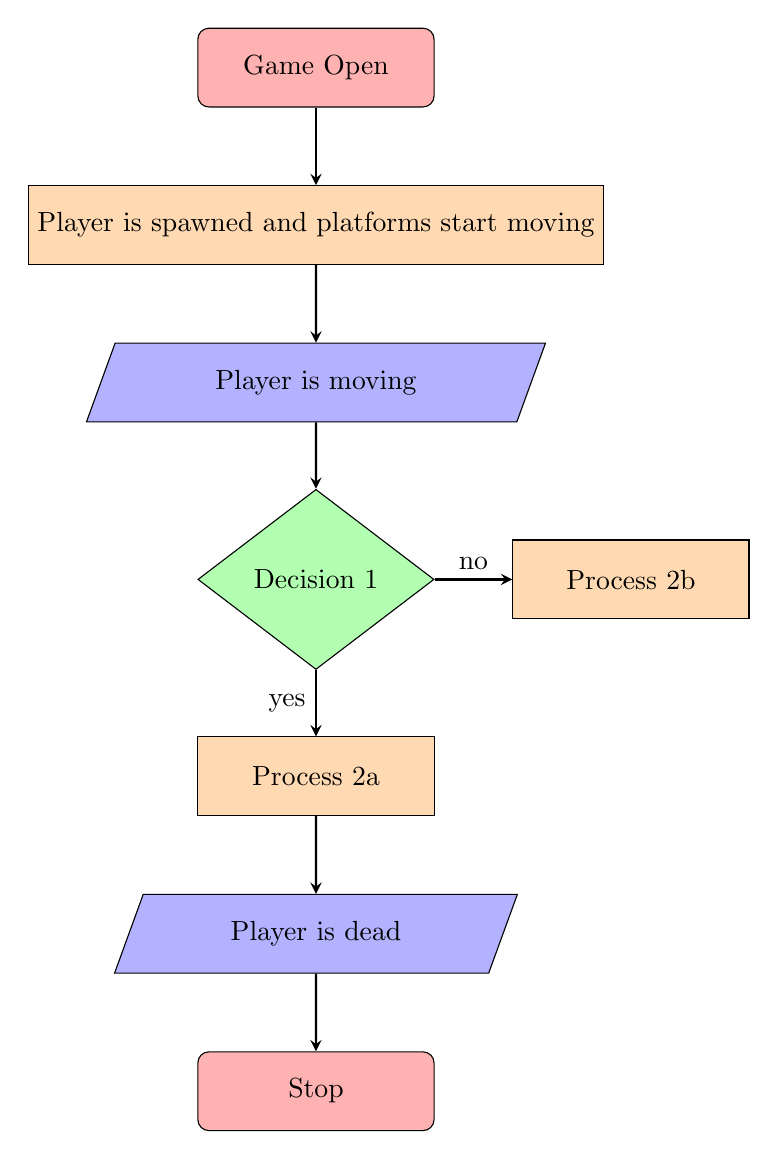
\begin{tikzpicture}[node distance=2cm]
	\node (start) [startstop] {Game Open};
	\node (proc1) [process, below of=start] {Player is spawned and platforms start moving};
	\node (in1) [io, below of=proc1] {Player is moving};
	\node (dec1) [decision, below of=in1, yshift=-0.5cm] {Decision 1};
	\node (proc2a) [process, below of=dec1, yshift=-0.5cm] {Process 2a};
	\node (proc2b) [process, right of=dec1, xshift=2cm] {Process 2b};
	\node (out1) [io, below of=proc2a] {Player is dead};
	\node (stop) [startstop, below of=out1] {Stop};
	\draw [arrow] (start) -- (proc1);
	\draw [arrow] (proc1) -- (in1);
	\draw [arrow] (in1) -- (dec1);
	\draw [arrow] (dec1) -- node[anchor=east] {yes} (proc2a);
	\draw [arrow] (dec1) -- node[anchor=south] {no} (proc2b);
	\draw [arrow] (proc2a) -- (out1);
	\draw [arrow] (out1) -- (stop);
	
\end{tikzpicture}

include diagrams to give evidence about the structure for the game. Give clear definition of objectives of the game. Flow chart showing the flow of the game through single or multiple layers with single or multiple players.

Include visualisation or written planetary designs or a combination of both and including alternatives, together with diagrams such as flowcharts.






\section{M2 Prepare alternative interface designs for the identified game concept}
Prepare alternative interface designs to the one identified in P3. The alternative designs must contain enough detail to enable them to be understood by a third party. Evidence can be extension of P3 and be presented as additional visualisations or written explanatory designs, or a combination of both.




\section{D1 Justify the design rational for the identified game concept}


\subsection{Original requirements}
To justify the design choices in our game we must first explcitly spell out the requirements as they were given to us

\begin{itemize}
\item The whole game experience must be familiar and easy to get to understand
\item The UX must not be confusing
\item Must work on all devices
\item Must be appealing to a younger audience
\item Players must have seen the likes of the game before
\item It must be small in scale, there will only be five levels
\item It must be engaging
\item It will have the clients food products
\item It will have monsters that must be defeated
\item It will educate players about the variety of foods, highlighting their unique qualities
\item Health boosts should be in the game based on their food products
\item As the player progresses through the levels, each level will become harder
\item There will be obstacles in the players way which must an navigated around. These should present moderately hard puzzles
\item On completion of the game the player is rewarded with a lifetime supply of the client's food
\end{itemize}

We will work through these one at a time

\subsection{ The whole game experience must be familiar and easy to get to understand }
This requirement is probably the one that has the largest impact on the game. It has made the design of the game a lot easier and quicker to develop as it has restricted us from try to deisgn a modern AAA game and instead we have been able to take a much more retro approach to designing the game. The logic behind this has been that as games from an earlier age of video games has been around a long time and almost everyone will have experienced these style of games in one form or another. 
This left the decsion as to which style of retro game to use. Games like Space Invaders and Pong, while they are arguably the grandfather of all modern games, they are not so well known in modern times and their gameplay mechanics is likely less understandable to a younger generation. Games of that era tended to be a bit more archiac. 
Moving on to games such a Pacman, Frogger, etc are also more well known but are a little too simplistic to provide an engaging and interesting gameplay.
Slightly more modern games such as Super Mario Brothers are much more well known and understood without have to have any preamble to explain what is happening. It was felt that it was too tempting to make this game as universal as it could be by using a side scrolling 2D platformer, so this is what we decided to go for. It not only means that it will be familiar, but there will also be very little friction for users starting to play the game. We will need to play test the game at an early stage with younger audiences but we are confident that they will have no problems understanding the mechanics.
 
\subsection{ The UX must not be confusing }
Making the user interface experience not be confusing also partially ties in to the requirement that the game must be familiar. It however goes furhter than that. We have decdided to use standard controls, as these are well known and very simple it means that this part of the game should be intuitive.

\subsection{ Must work on all devices }
\subsection{ Must be appealing to a younger audience }
\subsection{ Players must have seen the likes of the game before }
\subsection{ It must be small in scale, there will only be five levels }
\subsection{ It must be engaging }
\subsection{ It will have the clients food products }
\subsection{ It will have monsters that must be defeated }
\subsection{ It will educate players about the variety of foods, highlighting their unique qualities }
\subsection{ Health boosts should be in the game based on their food products }
\subsection{ As the player progresses through the levels, each level will become harder }
\subsection{ There will be obstacles in the players way which must an navigated around. These should present moderately hard puzzles }
Moving platofrm
Falling platofrm
Trap box

\subsection{ On completion of the game the player is rewarded with a lifetime supply of the client's food }


\end{document}
